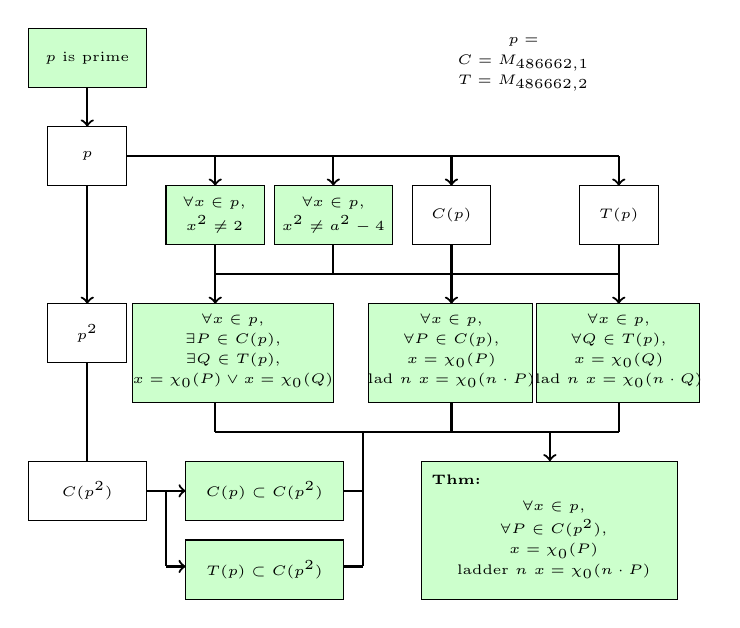
\begin{tikzpicture}[textstyle/.style={black, anchor= south west, align=center, minimum height=0.45cm, text centered, font=\tiny}]

  \draw (6.75,1) node[textstyle, anchor=north east] {$p = \p$\\[.6ex]$C = M_{486662,1}$\\[.6ex]$T = M_{486662,2}$};

  \begin{scope}[yshift=1 cm,xshift=-0.5 cm]
    \draw [fill=green!20] (0,0) -- (1.5,0) -- (1.5,-0.75) -- (0, -0.75) -- cycle;
    \draw (0.75,-0.375) node[textstyle, anchor=center] {$p$ is prime};
  \end{scope}

  \begin{scope}[yshift=-0.25 cm,xshift=-0.5 cm]
    \draw[fill=white] (0.25,0) -- (1.25,0) -- (1.25,-0.75) -- (0.25, -0.75) -- cycle;
    \draw (0.75,-0.375) node[textstyle, anchor=center] {$\F{p}$};
  \end{scope}

  \begin{scope}[yshift=-1 cm,xshift=1.25 cm]
    \draw[fill=green!20] (0,0) -- (1.25,0) -- (1.25,-0.75) -- (0, -0.75) -- cycle;
    \draw (0.615,-0.375) node[textstyle, anchor=center] {$\forall x \in \F{p},$\\[.6ex]$x^2 \neq 2$};
  \end{scope}

  \begin{scope}[yshift=-1 cm,xshift=2.625 cm]
    \draw[fill=green!20] (0,0) -- (1.5,0) -- (1.5,-0.75) -- (0, -0.75) -- cycle;
    \draw (0.75,-0.375) node[textstyle, anchor=center] {$\forall x \in \F{p},$\\[.6ex]$x^2 \neq a^2-4$};
  \end{scope}

  \begin{scope}[yshift=-1 cm,xshift=4.375 cm]
    \draw[fill=white] (0,0) -- (1,0) -- (1,-0.75) -- (0, -0.75) -- cycle;
    \draw (0.5,-0.375) node[textstyle, anchor=center] {$C(\F{p})$};
  \end{scope}

  \begin{scope}[yshift=-1 cm,xshift=6.5 cm]
    \draw[fill=white] (0,0) -- (1,0) -- (1,-0.75) -- (0, -0.75) -- cycle;
    \draw (0.5,-0.375) node[textstyle, anchor=center] {$T(\F{p})$};
  \end{scope}

  \path [thick, double, ->] (0.25,0.25) edge  [out=-90, in=90] (0.25,-0.25);
  \path [thick, double]     (0.75,-0.625) edge  [out=0, in=180] (7,-0.625);
  \path [thick, double, ->] (1.875,-0.625) edge  [out=-90, in=90] (1.875,-1);
  \path [thick, double, ->] (3.375,-0.625) edge  [out=-90, in=90] (3.375,-1);
  \path [thick, double, ->] (4.875,-0.625) edge  [out=-90, in=90] (4.875,-1);
  \path [thick, double, ->] (7,-0.625) edge  [out=-90, in=90] (7,-1);


  \begin{scope}[yshift=-2.5 cm,xshift=1.35 cm]
    \draw[fill=green!20] (-0.53,0) -- (2.03,0) -- (2.03,-1.25) -- (-0.53, -1.25) -- cycle;
    \draw (0.75,0) node[textstyle, anchor=north] {$\forall x \in \F{p},$\\[.6ex]$\exists P \in C(\F{p}),$\\[.6ex]$\exists Q \in T(\F{p})$,\\[.6ex]$x = \chi_0(P)\vee x = \chi_0(Q)$};
  \end{scope}

  \begin{scope}[yshift=-2.5 cm,xshift=4.125 cm]
    \draw[fill=green!20] (-0.3,0) -- (1.78,0) -- (1.78,-1.25) -- (-0.3, -1.25) -- cycle;
    \draw (0.75,0) node[textstyle, anchor=north] {$\forall x \in \F{p},$\\[.6ex]$\forall P \in C(\F{p}),$\\[.6ex]$x = \chi_0(P)\implies$\\[.6ex]lad $n$ $x = \chi_0(n \cdot P)$};
  \end{scope}

  \begin{scope}[yshift=-2.5 cm,xshift=6.25 cm]
    \draw[fill=green!20] (-0.3,0) -- (1.78,0) -- (1.78,-1.25) -- (-0.3, -1.25) -- cycle;
    \draw (0.75,0) node[textstyle, anchor=north] {$\forall x \in \F{p},$\\[.6ex]$\forall Q \in T(\F{p}),$\\[.6ex]$x = \chi_0(Q)\implies$\\[.6ex]lad $n$ $x = \chi_0(n \cdot Q)$};
  \end{scope}

  \path [thick, double, ->] (1.875,-1.75) edge  [out=-90, in=90] (1.875,-2.5);
  \path [thick, double]     (1.875,-2.125) edge  [out=0, in=180] (7,-2.125);
  \path [thick, double]     (3.375,-1.75) edge  [out=-90, in=90] (3.375,-2.125);
  \path [thick, double, ->] (4.875,-1.75) edge  [out=-90, in=90] (4.875,-2.5);
  \path [thick, double, ->] (7,-1.75) edge  [out=-90, in=90] (7,-2.5);

  % F(p^2)

  \path [thick, double, ->] (0.25,-1) edge  [out=-90, in=90] (0.25,-2.5);

  \begin{scope}[yshift=-2.5 cm,xshift=-0.5 cm]
    \draw[fill=white] (0.25,0) -- (1.25,0) -- (1.25,-0.75) -- (0.25, -0.75) -- cycle;
    \draw (0.75,-0.375) node[textstyle, anchor=center] {$\F{p^2}$};
  \end{scope}

  \path [thick, double, ->] (0.25,-3.25) edge  [out=-90, in=90] (0.25,-5);

  % C(F(p^2))

  \begin{scope}[yshift=-4.5 cm,xshift=-0.5 cm]
    \draw[fill=white] (0,0) -- (1.5,0) -- (1.5,-0.75) -- (0, -0.75) -- cycle;
    \draw (0.75,-0.375) node[textstyle, anchor=center] {$C(\F{p^2})$};
  \end{scope}

  \begin{scope}[yshift=-4.5 cm,xshift=1.5 cm]
    \draw[fill=green!20] (0,0) -- (2,0) -- (2,-0.75) -- (0, -0.75) -- cycle;
    \draw (1,-0.375) node[textstyle, anchor=center] {$C(\F{p}) \subset C(\F{p^2})$};
  \end{scope}

  \begin{scope}[yshift=-5.5 cm,xshift=1.5 cm]
    \draw[fill=green!20] (0,0) -- (2,0) -- (2,-0.75) -- (0, -0.75) -- cycle;
    \draw (1,-0.375) node[textstyle, anchor=center] {$T(\F{p}) \subset C(\F{p^2})$};
  \end{scope}

  \path [thick, double, ->] (1,-4.875) edge [out=0, in=-180] (1.5,-4.875);
  \path [thick, double] (1.25,-4.875) edge [out=-90, in=90] (1.25,-5.835);
  \path [thick, double, ->] (1.25,-5.835) edge [out=0, in=-180] (1.5,-5.835);

  \begin{scope}[yshift=-4.5 cm,xshift=4.5 cm]
    \draw [fill=green!20] (0,0) -- (3.25,0) -- (3.25,-1.75) -- (0, -1.75) -- cycle;
    \draw (0,0) node[textstyle, anchor=north west] {\textbf{Thm:}};
    \draw (1.675,-0.375) node[textstyle, anchor=north] {$\forall x \in \F{p},$\\[.6ex]$\forall P \in C(\F{p^2}),$\\[.6ex]$x = \chi_0(P)\implies$\\[.6ex]ladder $n$ $x = \chi_0(n \cdot P)$};
  \end{scope}

  \path [thick, double]     (1.875,-4.125) edge  [out=0, in=180] (7,-4.125);
  \path [thick, double]     (1.875,-3.75) edge  [out=-90, in=90] (1.875,-4.125);
  \path [thick, double]     (4.875,-3.75) edge  [out=-90, in=90] (4.875,-4.125);
  \path [thick, double]     (7,-3.75) edge  [out=-90, in=90] (7,-4.125);

  \path [thick, double]     (3.5,-4.875) edge  [out=0, in=180] (3.75,-4.875);
  \path [thick, double]     (3.5,-5.835) edge  [out=0, in=180] (3.75,-5.835);
  \path [thick, double]     (3.75,-5.835) edge  [out=90, in=-90] (3.75,-4.125);

  \path [thick, double, ->] (6.125,-4.125) edge [out=-90, in=90] (6.125,-4.5);

\end{tikzpicture}
